\documentclass[tikz]{standalone}% 'crop' is the default for v1.0, before it was 'preview'
\usepackage{tikz}
\usepackage{pgfplots}
\usepackage{amsmath}

\usepgfplotslibrary{colormaps}
\pgfplotsset{compat=1.18}
\usetikzlibrary{plotmarks, arrows.meta}
%\usetikzlibrary{...}% tikz package already loaded by 'tikz' option
\begin{document}


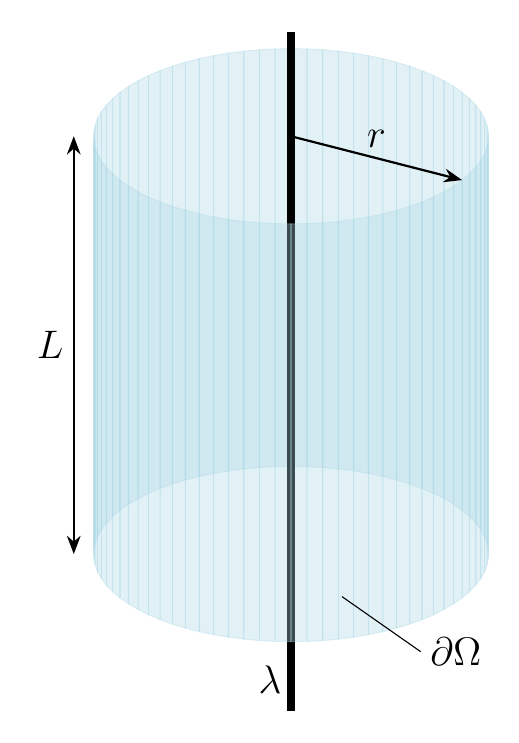
\begin{tikzpicture}[font=\Large]
  \begin{axis}[
    view={120}{40},
    hide axis,
    scale=2,
    xmin=-2, xmax=2, ymin=-2, ymax=2, zmin=0, zmax=4,
  ]

    % Parameters
    % radius r, angle theta, height z
    \addplot3[
      surf,                % draw a surface
      shader=flat,          % solid colour (no shading gradient)
      opacity=0.35,         % see-through
      samples=40,           % along theta
      samples y=2,          % along z (2 is enough for a true straight surface)
      domain=90:270,         % theta in degrees
      y domain=0:4,         % z range (height)
      draw=none,            % no mesh lines on the surface
      colormap={cyl}{
        rgb255(0cm)=(173,216,230); rgb255(1cm)=(173,216,230)
      }
    ] ({cos(x)}, {sin(x)}, {y}); % r=1 here

    % Line charge (vertical line)
    \addplot3[line width=3pt, color=black]
      coordinates {(0,0,-1.5) (0,0,5)};  % vertical line through origin
    \node[left] at (axis cs:0,0,-1.2) {$\lambda$};
\
    % radius r, angle theta, height z
    \addplot3[
      surf,                % draw a surface
      shader=flat,          % solid colour (no shading gradient)
      opacity=0.35,         % see-through
      samples=40,           % along theta
      samples y=2,          % along z (2 is enough for a true straight surface)
      domain=-90:90,         % theta in degrees
      y domain=0:4,         % z range (height)
      draw=none,            % no mesh lines on the surface
      colormap={cyl}{
        rgb255(0cm)=(173,216,230); rgb255(1cm)=(173,216,230)
      }
    ] ({cos(x)}, {sin(x)}, {y}); % r=1 here

    \draw[thick, <->, >=Stealth] (axis cs:{1.1*cos(60)}, {-1.1*sin(60)},0) -- (axis cs:{1.1*cos(60)},{-1.1*sin(60)},4) node[midway, left] {$L$};
    \draw[thick, ->, >=Stealth] (axis cs:0,0,4) -- (axis cs:0,1,4) node[midway, above] {$r$};
  \end{axis}

    \draw[thin, black] (8.5,1.8)  node[right] {$\partial \Omega$} -- (7.5,2.5);
\end{tikzpicture}
\end{document}